\documentclass[12pt,a4paper]{scrartcl}
\usepackage[utf8]{inputenc}
\usepackage[english,russian]{babel}
\usepackage{indentfirst}
\usepackage{misccorr}
\usepackage{graphicx}
\usepackage{amsmath}
\usepackage{multirow}
\usepackage{pgfplots}
\usepackage{diagbox}
\usepackage[top=1cm, bottom=1cm, left=1cm, right=1cm]{geometry}
\pgfplotsset{compat=1.9}

\begin{document}
	\graphicspath{{pic/}, {~/Pictures/TeXImgs/}}
	
	\newcommand{\ms}{\mathstrut}
	\newcommand{\msp}{\hspace{0.5cm}}
	\newcommand{\al}{\alpha}
	\newcommand{\dg}{^\circ}
	\newcommand{\qd}[2]{^{\frac{#1}{#2}}}
	\newcommand{\qdm}[2]{^{-\frac{#1}{#2}}}
	\newcommand{\lm}[2]{\underset{#1 \rightarrow #2}{\lim}}
	\newcommand{\sfrac}[2]{\dfrac{\strut #1}{\strut #2}}
	\newcommand{\equal}[1]{\overset{(#1)}{=}}
	\newcommand{\linevdots}{\ \raisebox{-.08\height}{\vdots}\ }
	\newcommand{\linecvdots}{\ \raisebox{-.08\height}{\vdots}\hspace{-0.13cm}\raisebox{.15\height}{\cancel{\phantom{a}}\hspace{0.06cm}}}
	\newcommand{\combox}[1]{\ms \msp \msp \begin{minipage}{0.95\linewidth}
			#1
	\end{minipage}}
	
	\newtheorem{pr}{Задача}
	\newtheorem{ex}{Пример}
	\newtheorem{dfn}{Def}
	\newtheorem{theorem}{Th}
	
	\newenvironment{slv}{\ms \msp \textit{Решение:}}{}
	\newenvironment{proof}{\ms \msp \textit{Доказательство: }}{\hfill $\square$}
	
	\begin{titlepage}
		
		\vspace*{\fill}
		
		\begin{center}
			
\includegraphics[scale=0.8]{MIPT.png}
			\\[0.7cm]\Huge Московский Физико-Технический Институт\\(национальный исследовательский университет)
			\\[2cm]\LARGE Отчет по эксперименту
			\\[0.5cm]\noindent\rule{\textwidth}{1pt}
			\\\Huge\textbf{Изучение колебаний струны}
			\\[-0.5cm]\noindent\rule{\textwidth}{1pt}
		\end{center}
		
		\begin{flushleft}
			\textit{Работа №1.4.5; дата: 22.11.21}\hfill\textit{Семестр: 1}
		\end{flushleft}
		
		\vspace*{\fill}
		
		\begin{flushleft}
			Выполнил: \hspace{\fill} Группа:
			\\Кошелев Александр \hspace{\fill} Б05-105
		\end{flushleft}
	\end{titlepage}
	
	%Страница 2
	
	\begin{flushleft}
		\footnotesize{Изучение колебаний струны} \hspace{\fill} \footnotesize{2}
		\\[-0.3cm]\noindent\rule{\textwidth}{0.3pt}
	\end{flushleft}
	
	\section{Аннотация}
	
	В данной работе изучаnuются поперечные, стоячие волны на тонкой натянутой струне; измеряются собственные частоты колебаний струны и проверяются условия образования стоячих волн; измеряются скорость распространения поперечных волн на струне и исследуется её зависимость от натяжения струны.
	
	\textbf{Схема установки:}
	\begin{center}
		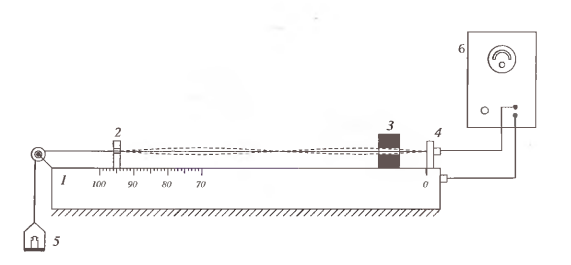
\includegraphics[scale=2]{PIC_1.png}
		\\\textbf{Рис. 1:} Схема установки
	\end{center}
	
	
	\textbf{В работе используются:} закрепленная на станине стальная струна, набор грузов, электромагнитные датчики, звуковой генератор, двухканальный осциллограф, частотомер.
	
	
	\section{Теоретические сведения}
	
	Пусть $F$ - сила натяжения струны, $\rho_l$ - погонная масса струны, $u$ - скорость распространения поперечной волны в струне. Тогда:
	
	\begin{equation}
		u = \sqrt{\sfrac{F}{\rho_l}}
	\end{equation}
	
	Зафиксируем частоту $\nu$. Тогда длина волны:
	
	\begin{equation}
		\lambda = \sfrac{u}{\nu}
	\end{equation}
	
	При этом на длине струны должно укладываться целое число полуволн $n$, тогда при длине струны $l$ из уравнения (2) получаем:
	
	\begin{equation}
		\nu_n = n \cdot \sfrac{u}{2l}
	\end{equation}

	\section{Проведение эксперимента}
	
	\paragraph{Визуальное наблюдение стоячих волн} \hfill
	
	\par При массе нагрузков $m = 1.1 \, \text{кг}$ будем медленно менять частоту звукового генератора в диапазоне $\nu=\nu_1 \pm 5$Гц и добьемся возбуждения стоячей волны на основной гармонике (одна пучность), а после и на больших гармнониках, и запишем результаты в Табл. 1 (удалось пронаблюдать 6 гармоник).
	
	%Страница 3
	
	\newpage
	
	\begin{flushleft}
		\footnotesize{Изучение колебаний струны} \hspace{\fill} \footnotesize{3}
		\\[-0.3cm]\noindent\rule{\textwidth}{0.3pt}
	\end{flushleft}
	
	\begin{center}
		\begin{tabular}{|c|c|}
			\hline
			$№$ & $\nu,\,\text{Гц}$   \\
			\hline 
			1 & 136.9 $\pm$ 0.1 \\
			\hline
			2 & 274.5 $\pm$ 0.1 \\
			\hline 
			3 & 413.7 $\pm$ 0.1 \\
			\hline
			4 & 550.1 $\pm$ 0.1 \\
			\hline
			5 & 688.4 $\pm$ 0.1 \\
			\hline
			6 & 831.2 $\pm$ 0.1 \\
			\hline
		\end{tabular}
		\\\textbf{Табл. 1: } Измерение частот прямым наблюдением
	\end{center}

	\paragraph{Регистрация стоячих волн с помощью осцилллографа} \hfill
	
	\par Будем изменять массу грузов, создающих натяжение струны, и измерять частоты различных гармоник при данной нагрузке с помощью осциллографа. Каждый раз будем проводить измерение частот 8 гармоник, так как на больших гармониках шумы слишком велики, и зафиксировать результат измерения частоты не представляется возможным. Частоты в герцах занесем в Табл. 2.
	
	\begin{center}
		\begin{tabular}{|c|c|c|c|c|c|}
			\hline
			\diagbox{№}{$T$, Н} & 7.02 $\pm$ 0.01 & 10.78 $\pm$ 0.01 & 15.33 $\pm$ 0.01 & 20.13 $\pm$ 0.01 & 24.99 $\pm$ 0.01
			\\\hline
			1 & 121.4 $\pm$ 0.1 & 137.6 $\pm$ 0.1 & 166.4 $\pm$ 0.1 & 190.1 $\pm$ 0.1 & 204.1 $\pm$ 0.1 
			\\\hline
			2 & 248.9 $\pm$ 0.1 & 277.8 $\pm$ 0.1 & 329.8 $\pm$ 0.1 & 379.3 $\pm$ 0.1 & 407.3 $\pm$ 0.1 
			\\\hline
			3 & 373.8 $\pm$ 0.1 & 416.5 $\pm$ 0.1 & 499.8 $\pm$ 0.1 & 566.0 $\pm$ 0.1 & 610.3 $\pm$ 0.1 
			\\\hline
			4 & 497.8 $\pm$ 0.1 & 551.1 $\pm$ 0.1 & 663.6 $\pm$ 0.1 & 748.6 $\pm$ 0.1 & 812.2 $\pm$ 0.1 
			\\\hline
			5 & 622.7 $\pm$ 0.1 & 690.9 $\pm$ 0.1 & 831.3 $\pm$ 0.1 & 935.1 $\pm$ 0.1 & 1020.4 $\pm$ 0.1 
			\\\hline
			6 & 746.4 $\pm$ 0.1 & 836.7 $\pm$ 0.1 & 998.3 $\pm$ 0.1 & 1124.3 $\pm$ 0.1 & 1224.7 $\pm$ 0.1 
			\\\hline
			7 & 886.5 $\pm$ 0.1 & 977.3 $\pm$ 0.1 & 1165.1 $\pm$ 0.1 & 1321.2 $\pm$ 0.1 & 1431.1 $\pm$ 0.1 
			\\\hline
			8 & 995.6 $\pm$ 0.1 & 1107.2 $\pm$ 0.1 & 1333.7 $\pm$ 0.1 & 1513.4 $\pm$ 0.1 & 1640.2 $\pm$ 0.1 
			\\\hline
		\end{tabular}
		\\\textbf{Табл. 2: } Измерение частот с помощью осциллографа
	\end{center}

	Построим графики зависимости частоты от номера гармоники по полученным данным. Для сравнения представим их на одном графике.
	
	\begin{center}
		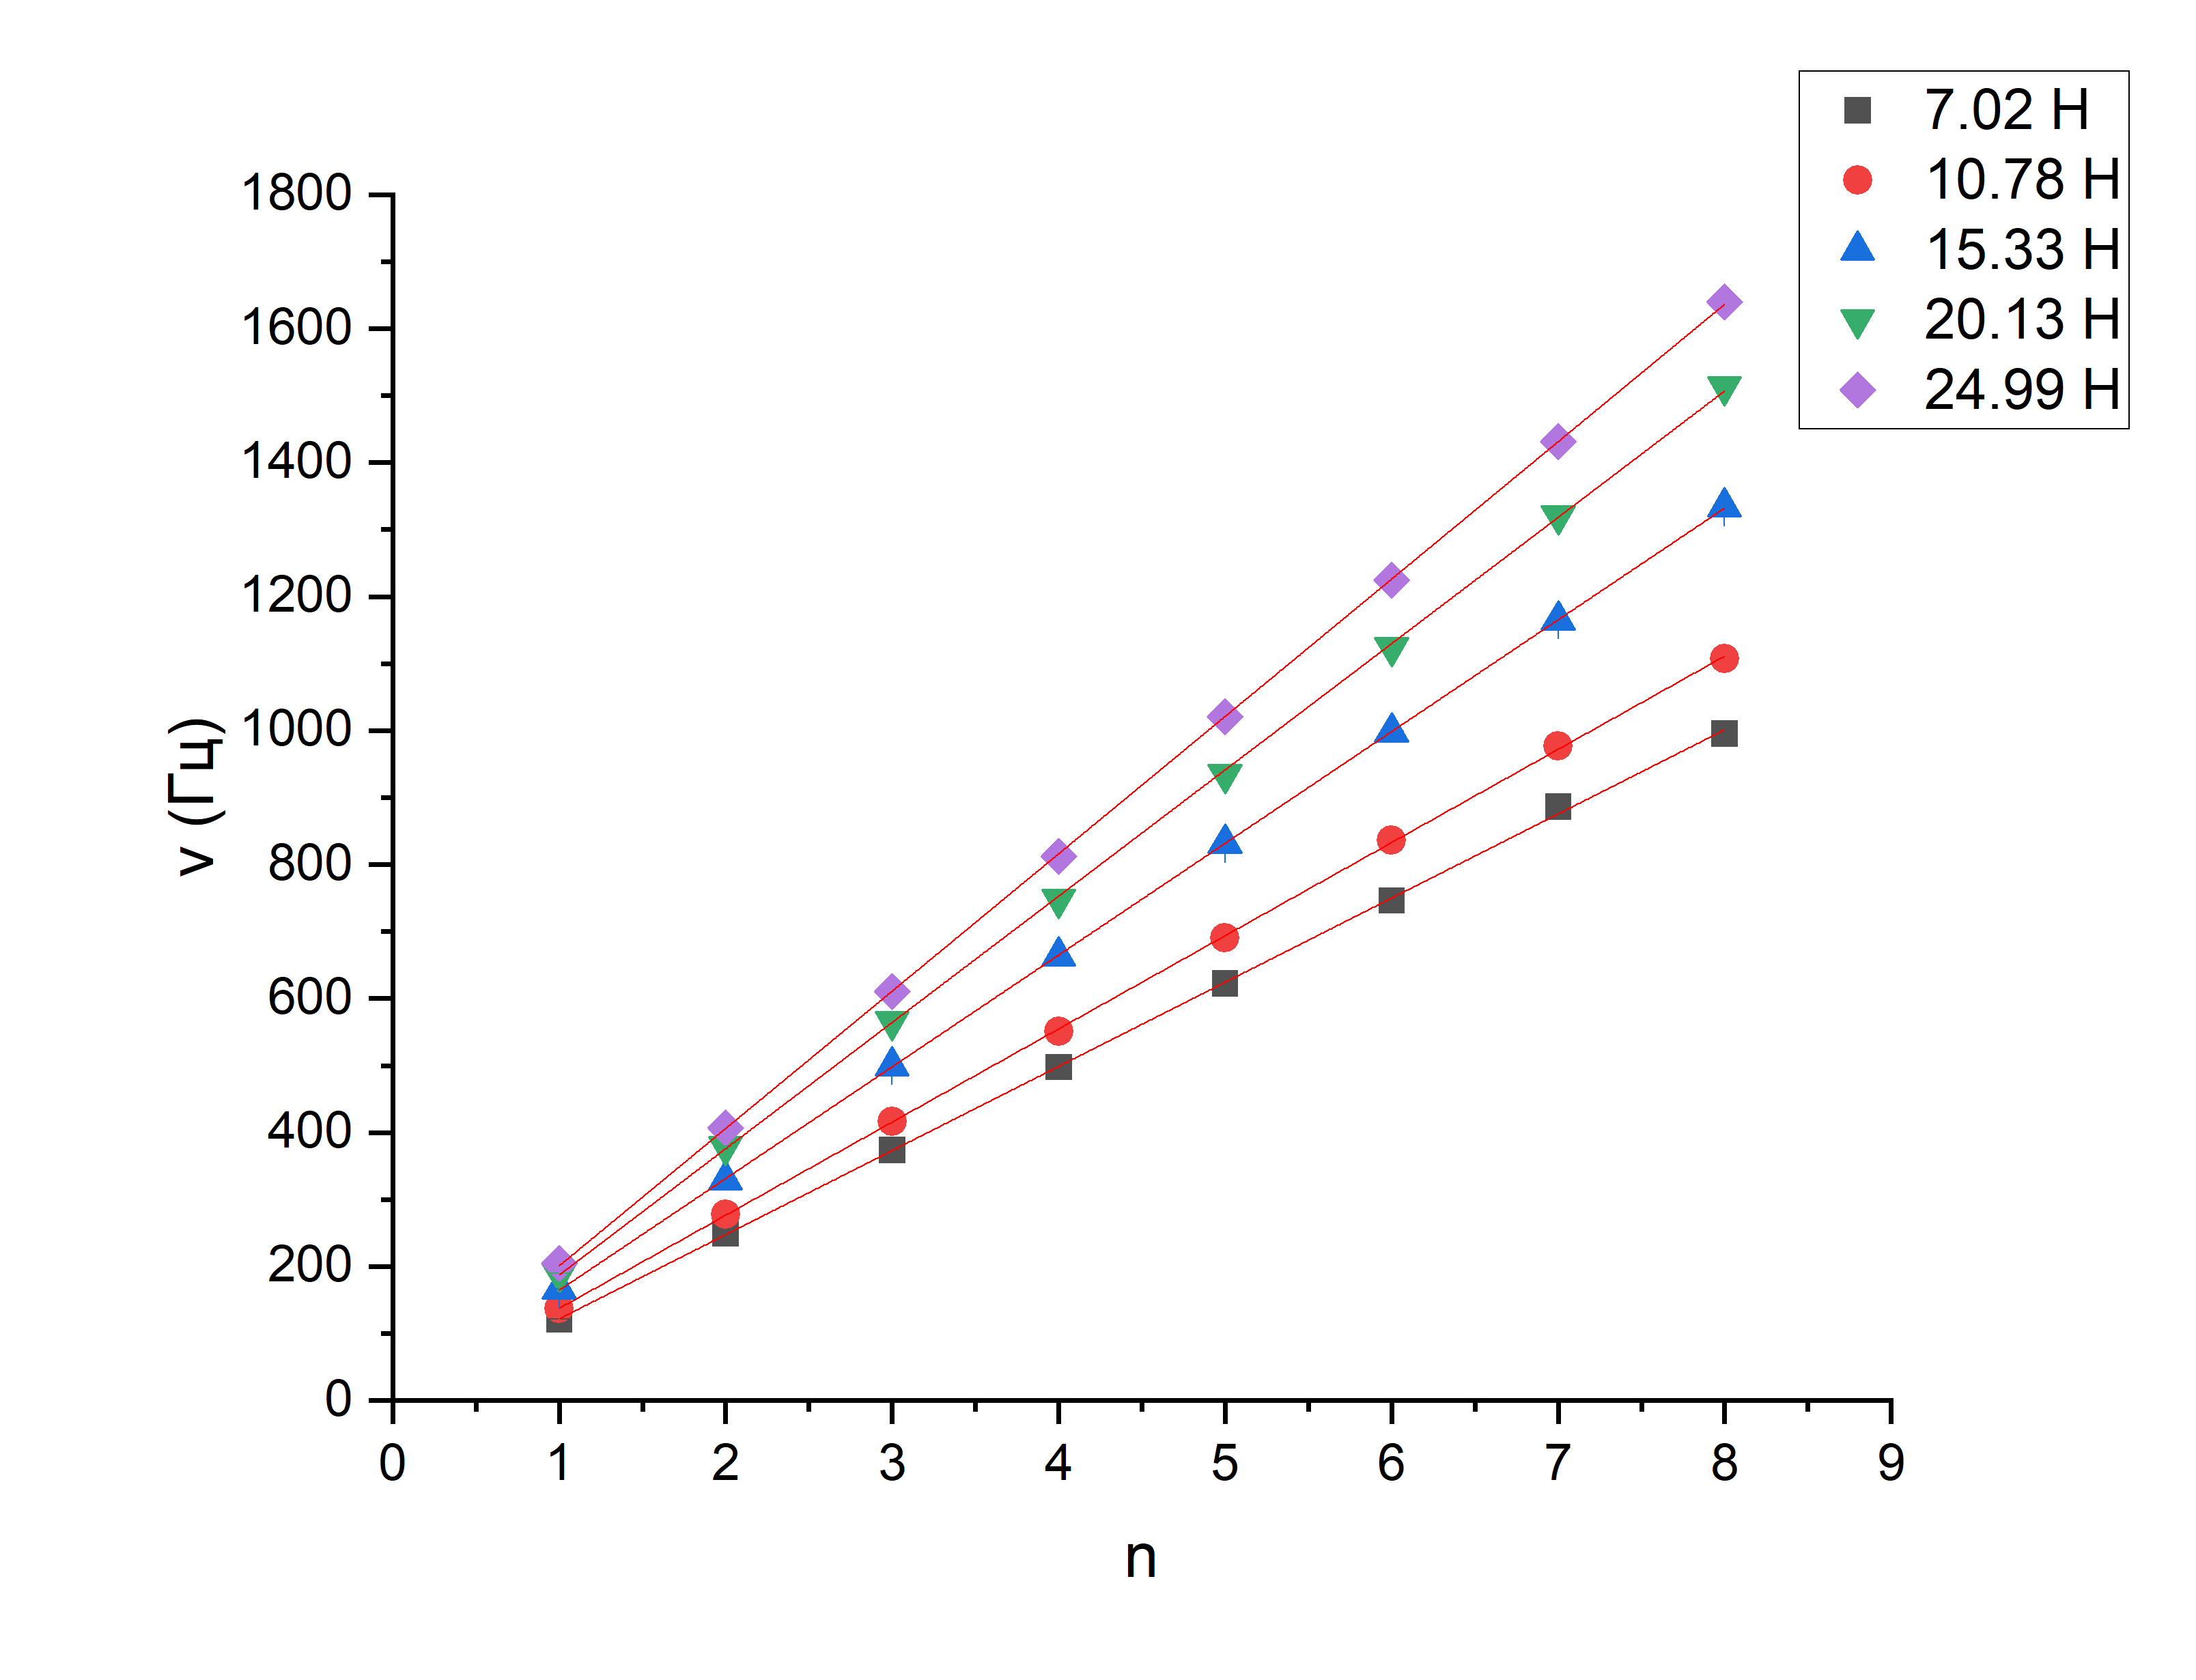
\includegraphics[scale=0.5]{PIC_2.png}
		\\\textbf{Рис. 2: } Графики зависимости $\nu(n)$
	\end{center}

	%Страница 4
	
	\newpage
	
	\begin{flushleft}
		\footnotesize{Изучение колебаний струны} \hspace{\fill} \footnotesize{4}
		\\[-0.3cm]\noindent\rule{\textwidth}{0.3pt}
	\end{flushleft}

	Обозначим коэффициенты наклона $\gamma$. Воспользовавшись формулой (3), выясняем:
	
	$$\gamma = \sfrac{\nu_n}{n} = \sfrac{u}{2l} \Rightarrow u = 2\gamma l$$
	
	Для нашей струны известна длина $l = 50\pm 0.5\,\text{см}$. Получим соответствующие $\gamma$ и $u$ для всех прямых при помощи линейной аппроксимации и занесем их в таблицу:
	
	\begin{center}
		\begin{tabular}{|c|c|c|c|c|c|}
			\hline
			$T$, Н & 7.02 $\pm$ 0.01 & 10.78 $\pm$ 0.01 & 15.33 $\pm$ 0.01 & 20.13 $\pm$ 0.01 & 24.99 $\pm$ 0.01
			\\\hline
			$\gamma$, с$^{-1}$ & 125.6 $\pm$ 0.8 & 139.1 $\pm$ 0.6 & 166.8 $\pm$ 0.2 & 188.5 $\pm$ 0.8 & 205.0 $\pm$ 0.42
			\\\hline
			$u$, м/с & 125.6 $\pm$ 1.5 & 139.1 $\pm$ 1.5 & 166.8 $\pm$ 1.7 & 188.5 $\pm$ 2.0 & 205.0 $\pm$ 2.1
			\\\hline
			$u^2$, (м/с)$^2$ & 15800 $\pm$ 400 & 19300 $\pm$ 400 & 27800 $\pm$ 600 & 35500 $\pm$ 800 & 42000 $\pm$ 900
			\\\hline
		\end{tabular}
		\\\textbf{Табл. 3: } Рассчет $u$
	\end{center}

	Теперь вспомним формулу (1) и определим зависимость между скоростью и натяжением:
	
	$$u^2 = \sfrac{T}{\rho_l} = \gamma'T$$
	
	Пусть $\gamma' = \rho_l^{-1}$ - коэффициент наклона зависимости $u^2(T)$. Построим график данной зависимости, определим $\gamma'$ и, наконец, получим погонную плотность струны:
	
	\begin{center}
		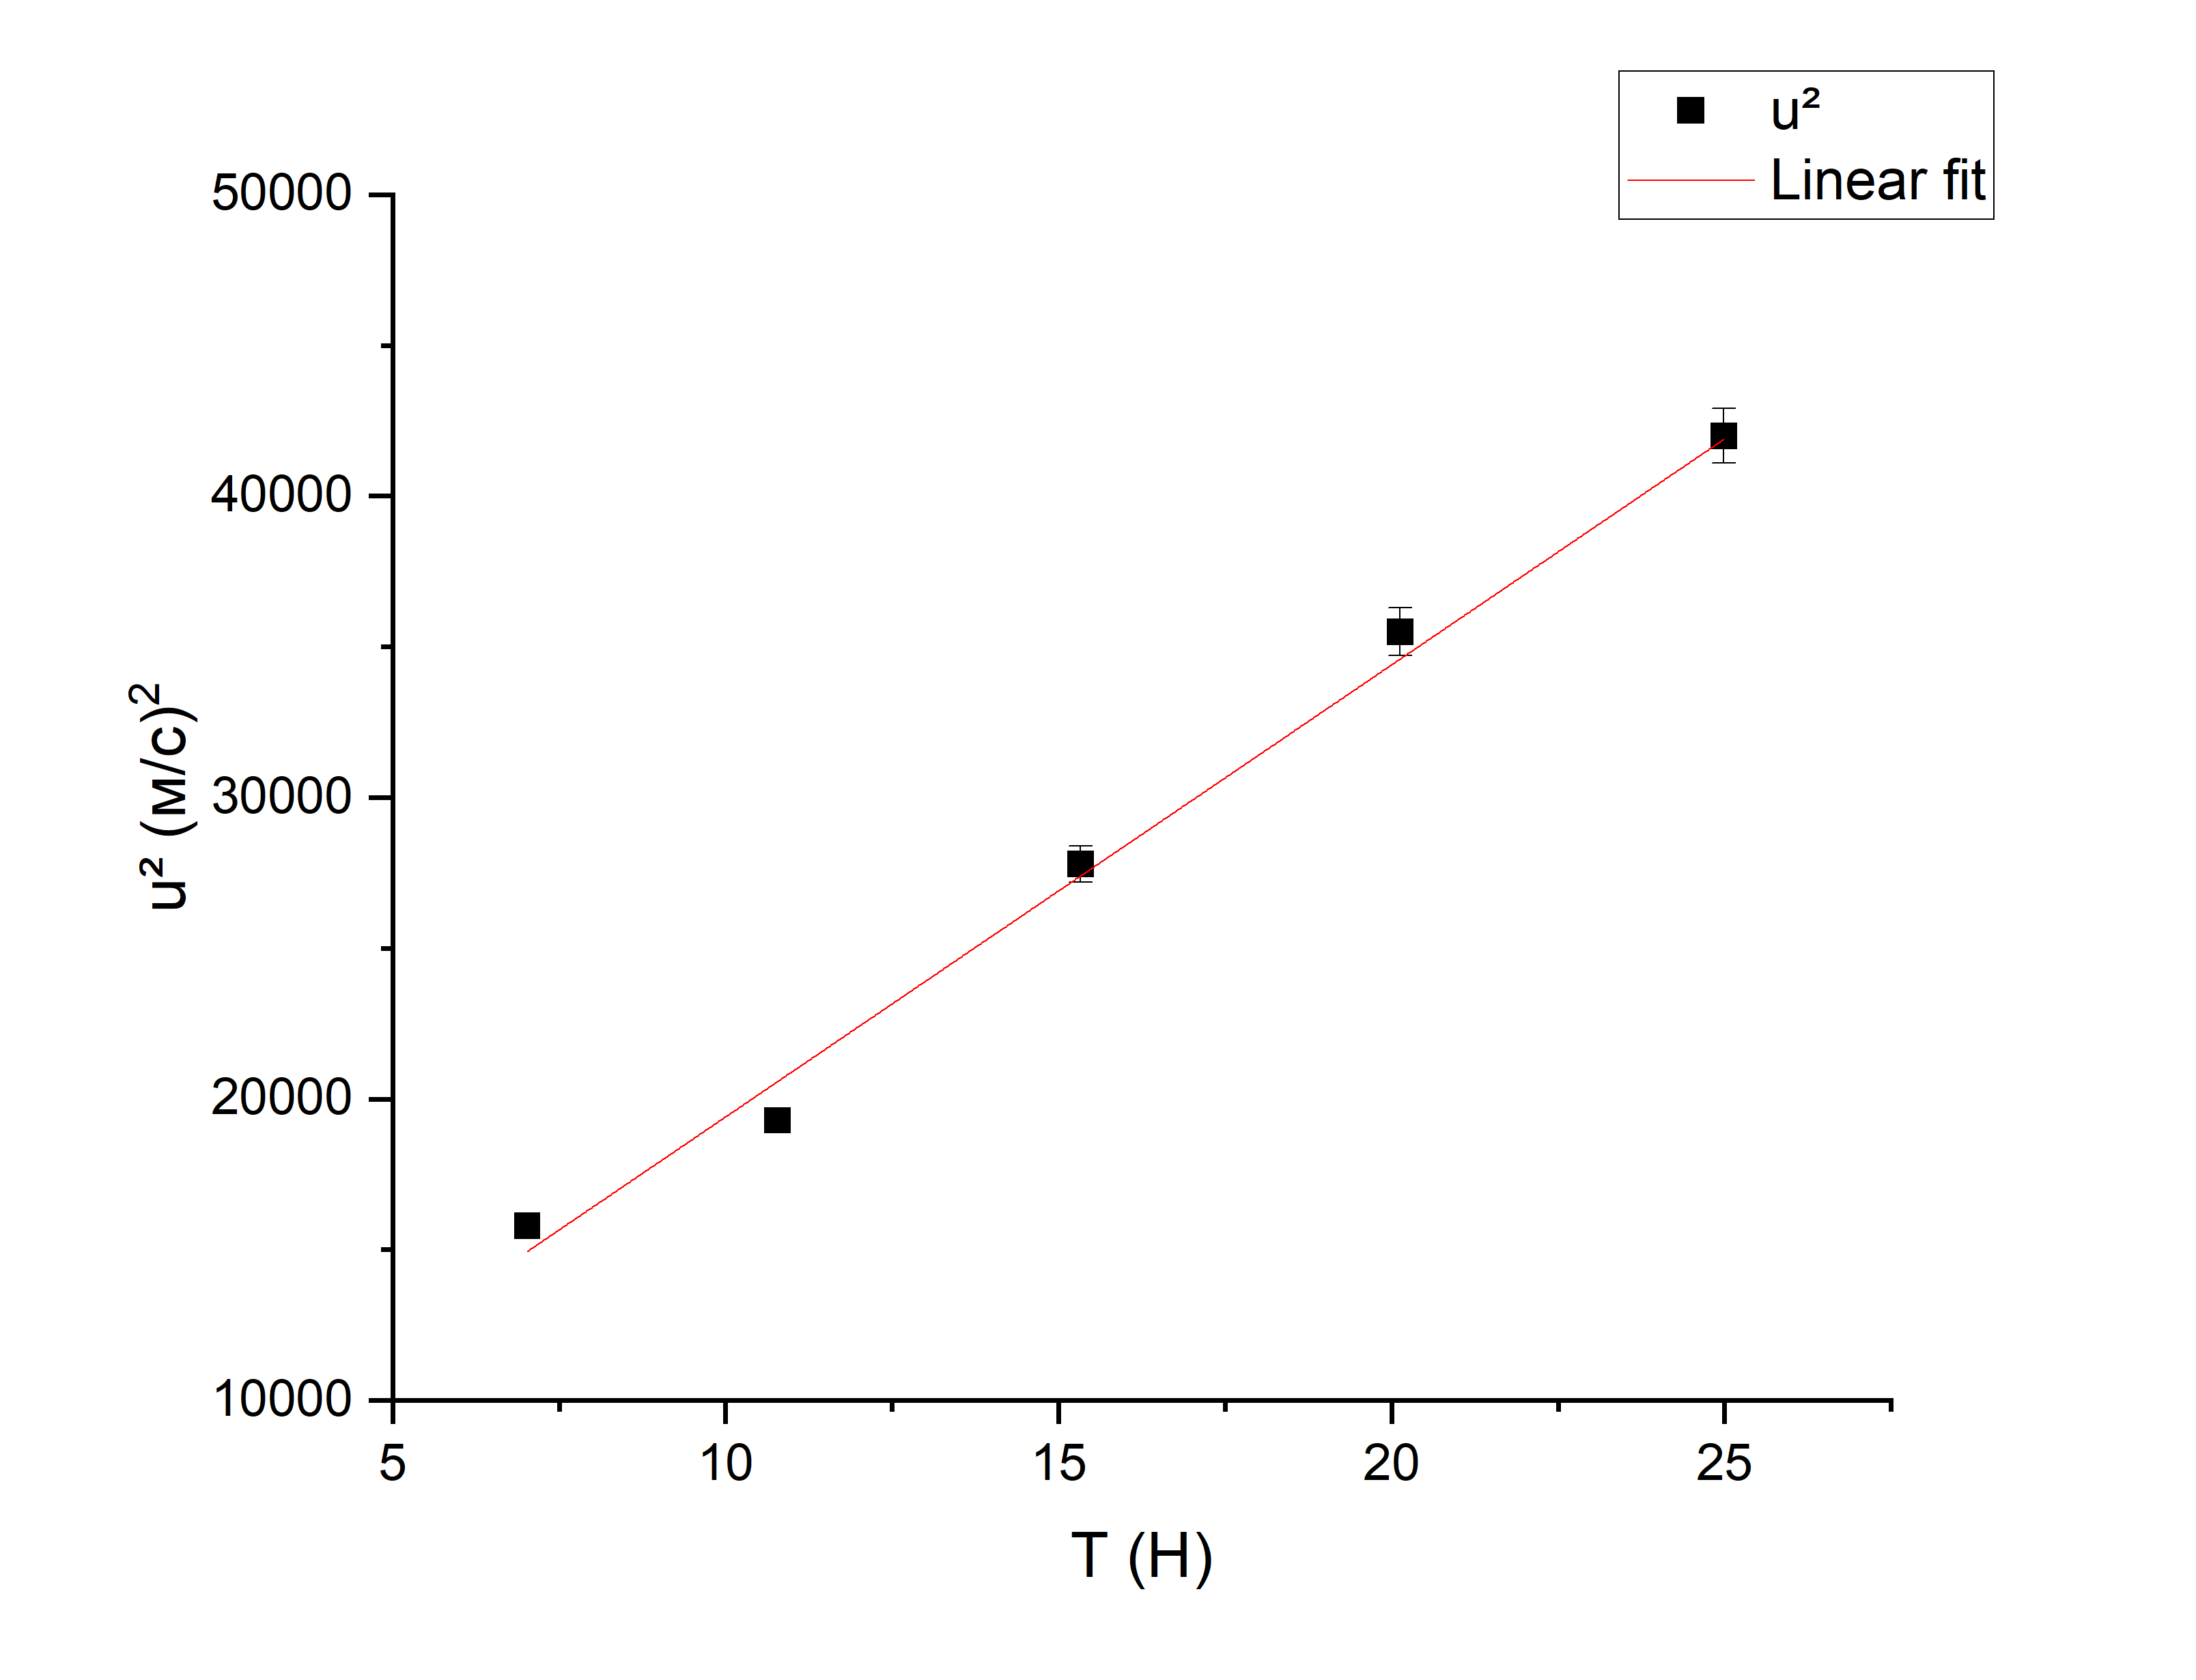
\includegraphics[scale=0.5]{PIC_3.png}
	\end{center}

	При помощи линейной аппроксимации:
	
	$$\gamma' = 1700 \pm 100\,\text{м/кг}$$
	
	$$\rho_l = (590 \pm 50) \,\text{мг/м}$$
	
	%Страница 5
	
	\newpage
	
	\begin{flushleft}
		\footnotesize{Изучение колебаний струны} \hspace{\fill} \footnotesize{5}
		\\[-0.3cm]\noindent\rule{\textwidth}{0.3pt}
	\end{flushleft}
	
	\section{Выводы}
		В работе было исследовано явление возникновения стоячих волн в струне. Установлено, что зависимость частоты гармоники от ее номера является линейной, а зависимость скорости звука в струне от натяжения струны - квадратичной. Было проверено условие возникновения стоячих волн в струне, а также определена погонная плотность струны:
		
		$$\rho_l = 590 \pm 50 \, \frac{\text{мг}}{\text{м}}$$
		
		Что хорошо (в пределах погрешности) согласуется со значением, полученным непосредственным взвешиванием:
		
		$$\rho_l = 568.4 \, \frac{\text{мг}}{\text{м}}$$.
		
		Отдельно отметим весьма большую погрешность полученной плотности. Такие значения следуют из метода наименьших квадратов. Для увеличения точности стоило бы провести большее количество измерений, что уменьшило бы стандартные отклонения.
\end{document}